% This is "sig-alternate.tex" V2.1 April 2013
% This file should be compiled with V2.5 of "sig-alternate.cls" May 2012
%
% This example file demonstrates the use of the 'sig-alternate.cls'
% V2.5 LaTeX2e document class file. It is for those submitting
% articles to ACM Conference Proceedings WHO DO NOT WISH TO
% STRICTLY ADHERE TO THE SIGS (PUBS-BOARD-ENDORSED) STYLE.
% The 'sig-alternate.cls' file will produce a similar-looking,
% albeit, 'tighter' paper resulting in, invariably, fewer pages.
%
% ----------------------------------------------------------------------------------------------------------------
% This .tex file (and associated .cls V2.5) produces:
%       1) The Permission Statement
%       2) The Conference (location) Info information
%       3) The Copyright Line with ACM data
%       4) NO page numbers
%
% as against the acm_proc_article-sp.cls file which
% DOES NOT produce 1) thru' 3) above.
%
% Using 'sig-alternate.cls' you have control, however, from within
% the source .tex file, over both the CopyrightYear
% (defaulted to 200X) and the ACM Copyright Data
% (defaulted to X-XXXXX-XX-X/XX/XX).
% e.g.
% \CopyrightYear{2007} will cause 2007 to appear in the copyright line.
% \crdata{0-12345-67-8/90/12} will cause 0-12345-67-8/90/12 to appear in the copyright line.
%
% -------------------------------------------------------------------------------------------------% For tracking purposes - this is V2.0 - May 2012

\documentclass{sig-alternate-05-2015}

\usepackage{url}                  % format URLs
\usepackage{listings}          % format code
\lstset{
  mathescape, 
  language={C},
  basicstyle=\small
}
\usepackage{enumitem}      % adjust spacing in enums
\usepackage[colorlinks=true,allcolors=blue,breaklinks,draft=false]{hyperref}   
\usepackage{graphicx}
\usepackage{float,subfig}
\usepackage{xspace,framed}
\usepackage{colortbl}
\usepackage{calc}

\usepackage{algorithm}
\usepackage{amsfonts}
\usepackage{multicol}
\usepackage{multirow}
\usepackage{tikz}
\usetikzlibrary{positioning, automata, shapes.arrows, calc, shapes, arrows}
\usepackage[justification=centering]{caption}
\usepackage{stmaryrd}
\usepackage{hhline}
\usepackage{pifont}
\usepackage{longtable}
\usepackage{afterpage}
\usepackage{wasysym}

\begin{document}

% Copyright
\setcopyright{acmcopyright}

% DOI
\doi{}

% ISBN
\isbn{}

%
% --- Author Metadata here ---
%\conferenceinfo{WOODSTOCK}{'97 El Paso, Texas USA}
%\CopyrightYear{2007} % Allows default copyright year (20XX) to be over-ridden - IF NEED BE.
%\crdata{0-12345-67-8/90/01}  % Allows default copyright data (0-89791-88-6/97/05) to be over-ridden - IF NEED BE.
% --- End of Author Metadata ---

\title{TBD}
%\subtitle{[Extended Abstract]
%\titlenote{A full version of this paper is available as
%\textit{Author's Guide to Preparing ACM SIG Proceedings Using
%\LaTeX$2_\epsilon$\ and BibTeX} at
%\texttt{www.acm.org/eaddress.htm}}}
%
% You need the command \numberofauthors to handle the 'placement
% and alignment' of the authors beneath the title.
%
% For aesthetic reasons, we recommend 'three authors at a time'
% i.e. three 'name/affiliation blocks' be placed beneath the title.
%
% NOTE: You are NOT restricted in how many 'rows' of
% "name/affiliations" may appear. We just ask that you restrict
% the number of 'columns' to three.
%
% Because of the available 'opening page real-estate'
% we ask you to refrain from putting more than six authors
% (two rows with three columns) beneath the article title.
% More than six makes the first-page appear very cluttered indeed.
%
% Use the \alignauthor commands to handle the names
% and affiliations for an 'aesthetic maximum' of six authors.
% Add names, affiliations, addresses for
% the seventh etc. author(s) as the argument for the
% \additionalauthors command.
% These 'additional authors' will be output/set for you
% without further effort on your part as the last section in
% the body of your article BEFORE References or any Appendices.

%\numberofauthors{8} %  in this sample file, there are a *total*
% of EIGHT authors. SIX appear on the 'first-page' (for formatting
% reasons) and the remaining two appear in the \additionalauthors section.
%
%% \author{
%% % You can go ahead and credit any number of authors here,
%% % e.g. one 'row of three' or two rows (consisting of one row of three
%% % and a second row of one, two or three).
%% %
%% % The command \alignauthor (no curly braces needed) should
%% % precede each author name, affiliation/snail-mail address and
%% % e-mail address. Additionally, tag each line of
%% % affiliation/address with \affaddr, and tag the
%% % e-mail address with \email.
%% %
%% % 1st. author
%% \alignauthor
%% Ben Trovato\titlenote{Dr.~Trovato insisted his name be first.}\\
%%        \affaddr{Institute for Clarity in Documentation}\\
%%        \affaddr{1932 Wallamaloo Lane}\\
%%        \affaddr{Wallamaloo, New Zealand}\\
%%        \email{trovato@corporation.com}
%% % 2nd. author
%% \alignauthor
%% G.K.M. Tobin\titlenote{The secretary disavows
%% any knowledge of this author's actions.}\\
%%        \affaddr{Institute for Clarity in Documentation}\\
%%        \affaddr{P.O. Box 1212}\\
%%        \affaddr{Dublin, Ohio 43017-6221}\\
%%        \email{webmaster@marysville-ohio.com}
%% }

\maketitle
\begin{abstract}

\end{abstract}


%
%  Use this command to print the description
%
\printccsdesc

% We no longer use \terms command
%\terms{Theory}

\keywords{}

%%%%%%%%%%%%%%%%%%%%%%%%%%%%%%%%%%%%%%%%%%%%%%%%%%%%%%%%%%%%%%%%%%%%%%%%%%%%%%%%%%%%%%
\section{Introduction}

We are interested in the stability of closed-loop systems, i.e.,
controllers along with a model of their physical environment, the
plant, as shown in Fig.~\ref{fig:closed-system}.

\begin{figure*}
\centering
\resizebox{.5\textwidth}{!}{
 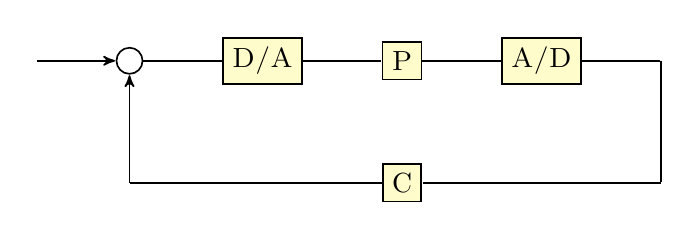
\begin{tikzpicture}[scale=0.3,-,>=stealth',shorten >=.2pt,auto,
     semithick, initial text=, ampersand replacement=\&,]

  \matrix[nodes={draw, fill=none, shape=rectangle, minimum height=.2cm, minimum width=.2cm, align=center}, row sep=1cm, column sep=1cm] {
   \coordinate (aux0);
   \& \node[circle] (circle) {}; 
   \& \node[fill=yellow!20] (da) {{\sc D/A}}; 
   \& \node[fill=yellow!20] (p) {{\sc P}};
   \& \node[fill=yellow!20] (ad) {{\sc A/D}}; 
   \& \coordinate (aux1);\\
   \& \coordinate (aux3); 
   \&
   \&
   \node[fill=yellow!20] (c) {C};
   \& 
   \& \coordinate (aux2);\\
  };


  \path[->] (aux0) edge (circle.west);
  \path  
   (circle.east) edge (da.west)
   (da.east) edge (p.west)
   (p.east) edge (ad.west)
   (ad.east) edge (aux1.west)
   (aux1.south) edge (aux2.north)
   (aux2.west) edge (c.east)
   (c.west) edge (aux3.east); 
  \path[->]  (aux3.north) edge (circle.south);
 \end{tikzpicture}
}
 \caption{Closed-Loop System. \label{fig:closed-system}}
\end{figure*}

%%%%%%%%%%%%%%%%%%%%%%%%%%%%%%%%%%%%%%%%%%%%%%%%%%%%%%%%%%%%%%%%%%%%%%%%%%%%%%%%%%%%%%
\section{Overview}
%%%%%%%%%%%%%%%%%%%%%%%%%%%%%%%%%%%%%%%%%%%%%%%%%%%%%%%%%%%%%%%%%%%%%%%%%%%%%%%%%%%%%%
\section{Running Example}


A classical cruise control example is extracted from the literature~\cite{Astrom08}, where the discrete plant model (with time step of $0.2$s) is represented by the following z-expression:

\begin{equation}
\label{Eq:running-example-plant}
P\left(z\right) := \frac{0.0264}{z-0.9998}.
\end{equation}

Using an optimization tool, Wang {\it et al.}~\cite{DBLP:conf/hybrid/WangGRJF16} design a high-performance controller, which is characterized by the following z-expression:

\begin{equation}
\label{Eq:running-example-controller}
C\left(z\right) := \frac{2.72z^2 - 4.153z + 1.896}{z^2 - 1.844z + 0.8496}.
\end{equation}

The authors claim that this controller $C(z)$ is extremely stable for the discrete plant model $P(z)$. However, if implementation aspects are considered during verification, this controller becomes unstable. To properly implement $C(z)$, there is a function $FWL[\cdot]:\mathbb{R}^{k+l+2}\rightarrow Q[\mathbb{R}^{k+l+2}]$, which applies FWL effects to the controller $C(z)$, where $Q[\mathbb{R}]$ represents the quantized set of representable real numbers in the chosen implementation format $<k,l>$ ($k$ is the number of bits of the integer part and $l$ is the number of bits of the fractional part). 

For this particular example, the actual implementation of $C(z)$ using $<3,16>$ implementation format can be represented by the following z-expression:

\begin{equation}
\label{Eq:running-example-controller-quantized}
C_{q}\left(z\right) := \frac{2.7199859619140625z^2 - 4.1529998779296875z + 1.89599609375}{z^2 - 1.843994140625z + 0.8495941162109375},
\end{equation} 

\noindent which makes the system unstable in closed-loop using series loop configuration.

%%%%%%%%%%%%%%%%%%%%%%%%%%%%%%%%%%%%%%%%%%%%%%%%%%%%%%%%%%%%%%%%%%%%%%%%%%%%%%%%%%%%%%
\section{Program Synthesis}

We use CounterExample-Guided Inductive Synthesis (CEGIS), as
illustrated in Fig~\ref{fig:CEGIS}.

\begin{figure*}
\centering
\resizebox{.7\textwidth}{!}{
 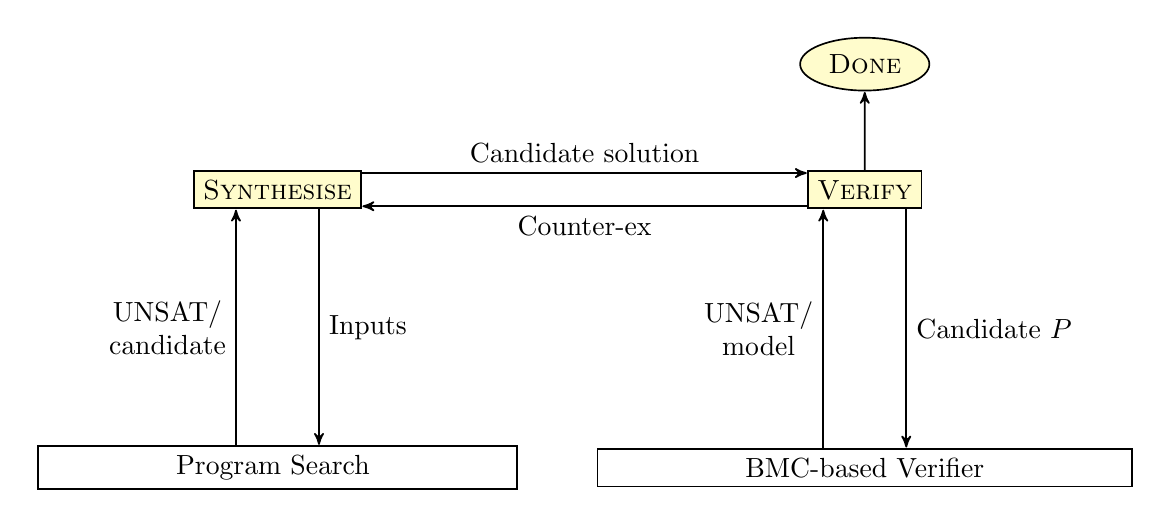
\begin{tikzpicture}[scale=0.3,->,>=stealth',shorten >=.2pt,auto, semithick, initial text=, ampersand replacement=\&,]
  \matrix[nodes={draw, fill=none, shape=rectangle, minimum height=.2cm, minimum width=.2cm, align=center
},
          row sep=1cm, column sep=1cm] {
   \& \node[ellipse, fill=yellow!20] (done) {{\sc Done}}; \\
   \node[fill=yellow!20] (synth) {{\sc Synthesise}};
   \&
   \node[fill=yellow!20] (verif) {{\sc Verify}}; \\

   \& \\
   \& \\
   \node (gp) {~~~~~~~~~~~~~~Program Search~~~~~~~~~~~~~~~};
   \&
   \node (bmc) {~~~~~~~~~~~~~~~BMC-based Verifier~~~~~~~~~~~~~~~};
   
    \\
  };

   \path
    ([yshift=2em]synth.east) edge node {Candidate solution} ([yshift=2em]verif.west)
    ([yshift=-2em]verif.west) edge node {Counter-ex} ([yshift=-2em]synth.east)
    ([xshift=5em]verif.south) edge node {Candidate $P$} ([xshift=5em]bmc.north)
    ([xshift=-5em]bmc.north) edge node[align=center]  {UNSAT/\\model} ([xshift=-5em]verif.south)
    (verif) edge node {} (done)
    ([xshift=5em]synth.south) edge node[align=center] {Inputs} ([xshift=5em]gp.north)
    ([xshift=-5em]gp.north) edge node[align=center] {UNSAT/\\candidate} ([xshift=-5em]synth.south);
 \end{tikzpicture}
}
 \caption{Counterexample-Guided Inductive Synthesis. \label{fig:CEGIS}}
\end{figure*}
%%%%%%%%%%%%%%%%%%%%%%%%%%%%%%%%%%%%%%%%%%%%%%%%%%%%%%%%%%%%%%%%%%%%%%%%%%%%%%%%%%%%%%
\section{Experiments}
%%%%%%%%%%%%%%%%%%%%%%%%%%%%%%%%%%%%%%%%%%%%%%%%%%%%%%%%%%%%%%%%%%%%%%%%%%%%%%%%%%%%%%
\section{Related Works}

\paragraph{Robust synthesis of Linear Systems} 

The problem of parametric control synthesis based on stability measures for continous Linear Time Invariant (LTI) Single Input-Single Output (SISO) systems has been researched for several decades. On a theoretical level it is a solved problem\cite{wonham1967pole} for which researches continuously seek better results based on a number of properties in addition to stability. A vast range of pole placement techniques such as Moore's algorithm for eigenstructure assignment \cite{klein1977eigenvalue} or the more recent Linear Quadratic Regulator (LQR) \cite{bemporad2002explicit} have been used in several papers with increasing degrees of succes to ensure stability. The latter approach highlights the importance of conserving energy during the control process, which results amongst other things in lower running costs. Since real systems are subject to tolerance and noise as well as the need for economy, more recent works focus on the problems of achieving robust stability with minimum gain \cite{schmid2014unified,konigorski2012pole}. 
However, when extending the problem to digital controller synthesis, many of these techniques lack the ability to produce sound or stable results because they disregard the effects of quantization and rounding. Modern papers on implementations/synthesis of LTI digital controllers \cite{das2013lqr,ghosh2013fpga} focus on time discretization, failing to account for these error-inducing effects and can therefore result in digitally unstable systems that have been proven to be robustly stable in a continuous space. This situation demands the inclusion of formal methods to verify the effects of space discretization on the implementation of the controller.

\paragraph{Formal Verification of Linear Digital Controllers} 

Researchers in formal verification methods of control systems have studied various effects of discretising the dynamics, including delayed response \cite{Duggirala2015}, and Finite Word Length (FWL) constraints with the objective to either verify (eg. \cite{daes20161}) or optimise (eg. \cite{oudjida2014design}) implementations. There are in fact two different problems arising from FWL effects. The first corresponds to the error in the dynamics caused by the inability of the hardware to represent the exact dynamics of the system whilst the second relates to rounding errors during computation. 
In \cite{fialho1994stability} a stability measure based on the error of the digital dynamics ensures that the FWL errors do not make the digital system unstable. A more recent approach \cite{DBLP:journals/automatica/WuLCC09} uses $\mu$ calculus to directly model the digital controller so that the selected parameters are stable by design. Most papers following this line of verification focus on finding a correct implementation of a known desired controller, looking for optimal parameter representations using FWL but ignoring the effects of rounding errors due to issues of mathematical tractability.
The analyses in \cite{DBLP:conf/hybrid/WangGRJF16,DBLP:conf/hybrid/RouxJG15} rely on an invariant computation on the discrete system dynamics using Semi-Definite Pogramming (SDP). Whilst the former uses BIBO properties to determine stability, the latter uses Lyapunov-based quadratic invariants. In both cases the SDP solver uses floating point arithmetic and soundness is checked by upper bounding the error.

\paragraph{Robust Synthesis of FWL Digital Controllers}

To the authors' knowledge, there is no existing work on the automatic synthesis of digital controllers considering FWL effects. Parameter synthesis tools such as \cite{cimatti2013parameter} use bounded model checking and fixed point computations to find parameters based on user defined specifications, but they often operate in the continuous domain and are ill-suited for robust analysis since they have no direct means of evaluating robustness. Other tools such as \cite{economakos2016automated} are directly aimed at robust stability problems but fail to explore the effects of FWL in their implementation.
In order to provide a correct by design controller, \cite{alur2016compositional} requires a user-defined finite state abstraction to synthesise a digital controller based on high level specifications. Whilst this approach directly overcomes the challenges presented by the FWL problem, it still requires error-prone user intervention. A different solution that looks at the other end of the scale is an approach that synthesises word lengths for know problems as developed in \cite{jha2013swati}, however this provides neither an optimal word synthesis nor a comprehensive solution for the problem.
It is from this vacuum that we seek to explore a CEGIS approach to FWL controller synthesis.

\paragraph{CEGIS}

In recent years the development of program synthesis has found many ways to obtain correct by design programs from high level specifiactions. One such approach \cite{itzhaky2010simple} looks to inductively synthesise invariants to generate the desired programs. Since these digital programs are already constrained by designed to factors such as FWL, these approaches are ideal for the synthesis of parametric controllers.
In \cite{DBLP:conf/cdc/RavanbakhshS15}, the authors use CEGIS for the synthesis of switching controllers for stabilizing continuous-time plants with polynomial dynamics. The work extends to its application on affine systems, finding its major challenge in the hardness of solving linear arithmetic on present SMT solvers. Since this approach uses switching states instead of linear dynamics in the digital controller, it entirely circumvents the FWL problem. It is also not suitable for the kind of control we seek to synthesise.
What is needed in this regard is the combination of a synthesis engine with a control verification tool that addresses the challenges presented here in the form of FWL effects and stability measures for LTI SISO controllers. We take the former from \cite{} and the latter from \cite{daes20161} whilst enhancing the procedure by evaluating the quantaization effects of the Hardware interfaces (ADC/DAC) to obtain an accurate discrete time FWL representation of the continuous dynamics.
 
%In \cite{DBLP:journals/corr/PakmehrWJVF13}, Pakmehr et al.  design a control software verification framework for gas turbine engines.

%%%%%%%%%%%%%%%%%%%%%%%%%%%%%%%%%%%%%%%%%%%%%%%%%%%%%%%%%%%%%%%%%%%%%%%%%%%%%%%%%%%%%%
\section{Conclusions}

\bibliographystyle{abbrv}
\bibliography{paper}  

%APPENDICES are optional
%\balancecolumns
%\appendix
%Appendix A
\end{document}
